\documentclass[fontset=windows]{article}

\usepackage{geometry}
\usepackage{float}
\usepackage{makecell}
\usepackage{amsmath}
\usepackage{ctex}
\usepackage{lastpage}%页数页眉宏包
\usepackage{abstract}%摘要宏包
\usepackage{indentfirst}%第一段空格
\usepackage{fancyhdr}
\usepackage{amssymb}
\usepackage{multicol}
\usepackage{multirow} 
\usepackage{amsmath}
\usepackage{amsthm}
\usepackage{graphicx}
\usepackage{subcaption}
\usepackage{cleveref}   %可以调用 \Cref{fig:xxx}或者 \ref{fig:xxx} 
\usepackage[linesnumbered,lined,boxed,commentsnumbered,ruled]{algorithm2e}
\usepackage{array}
\usepackage{listings}
\usepackage[usenames,dvipsnames]{xcolor}
\usepackage{color}


\title{图像处理与分析第一次作业}
\author{162050127颜劭铭}
\date{\zhtoday}

\begin{document}
\maketitle

    \section{计算并显示以下图像的直方图}

        矩阵操作进行计算

        \begin{figure}[H]
            \centering
            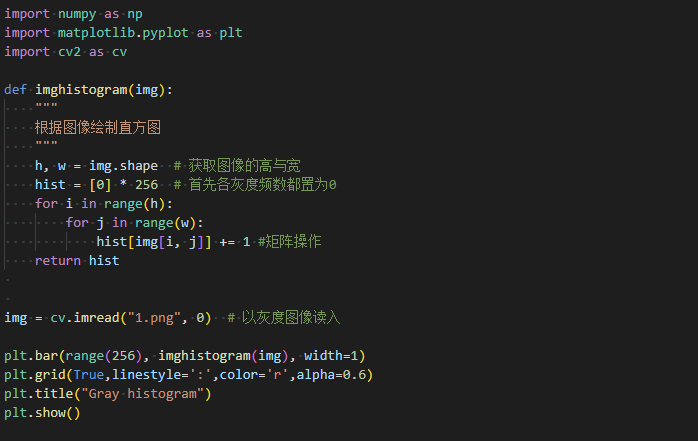
\includegraphics[scale=0.35]{code1.png}
            \caption{代码}
        \end{figure}

        \begin{figure}[H]
            \centering
            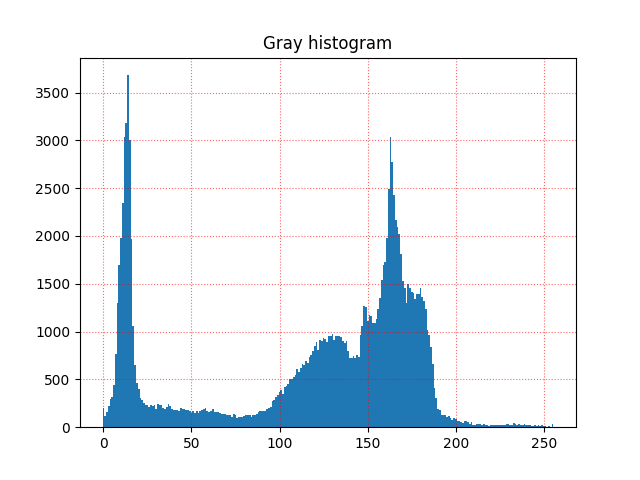
\includegraphics[scale=0.45]{Gray_histogram.png}
            \caption{结果}
        \end{figure}

    \section{2.分别对以下图片进行图像增强}

        \subsection{第一张}

            将RGB拆成R,G,B三个通道矩阵,分别对3通道进行直方图均衡化,然后合成为RGB图

            \begin{figure}[H]
                \centering
                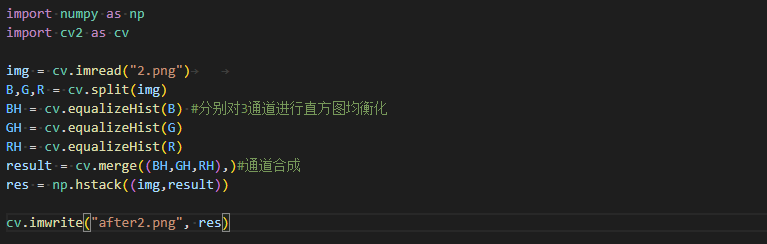
\includegraphics[scale=0.6]{code2.png}
                \caption{代码}
            \end{figure}

            \begin{figure}[H]
                \centering
                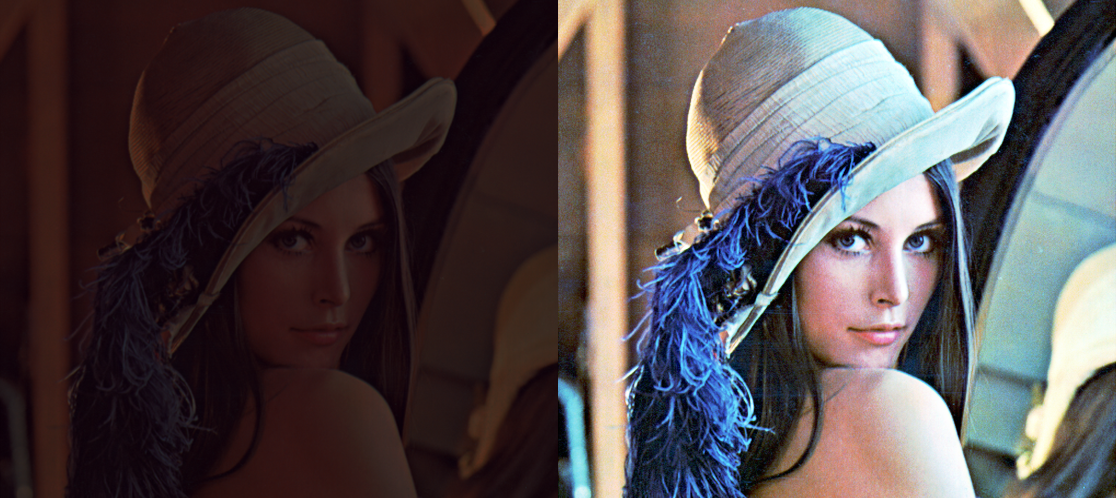
\includegraphics[scale=0.35]{after2.png}
                \caption{结果}
            \end{figure}

        \subsection{第二张}

            将RGB拆成R,G,B三个通道矩阵,分别对3通道进行直方图均衡化,然后合成为RGB图

            \begin{figure}[H]
                \centering
                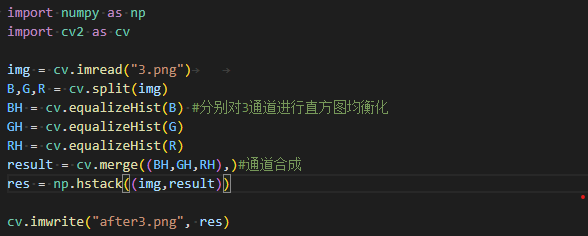
\includegraphics[scale=0.6]{code3.png}
                \caption{代码}
            \end{figure}

            \begin{figure}[H]
                \centering
                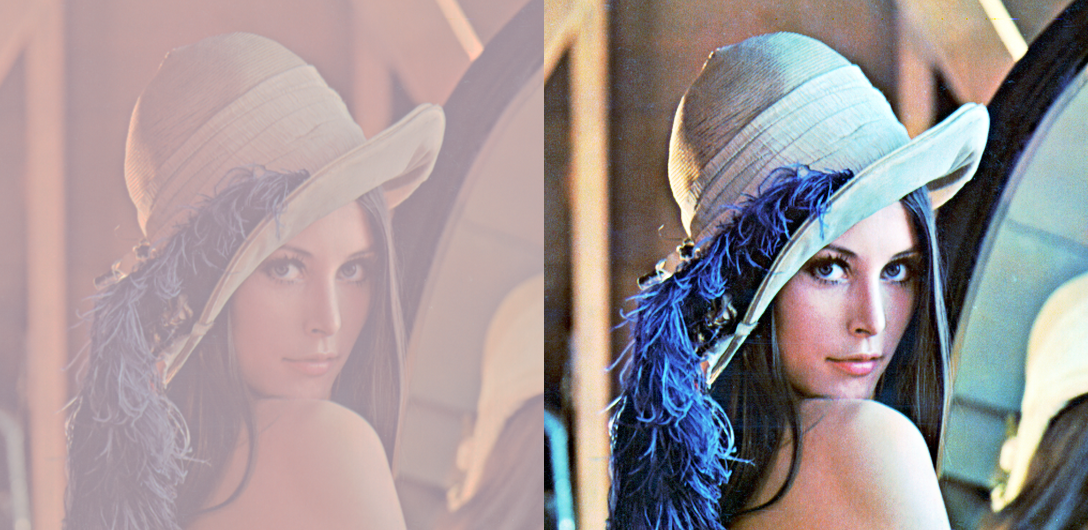
\includegraphics[scale=0.35]{after3.png}
                \caption{结果}
            \end{figure}

        \subsection{第三张}

            中值滤波,设置了不同滤波器大小,滤波器大小为$3 \times 3$的时候效果最好,噪点最少且不模糊 

            \begin{figure}[H]
                \centering
                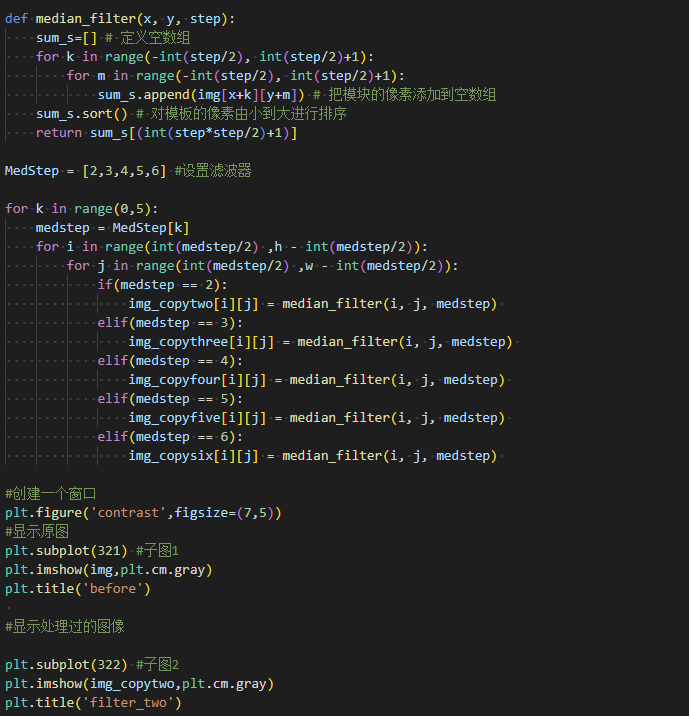
\includegraphics[scale=0.6]{code4.png}
                \caption{代码}
            \end{figure}

            \begin{figure}[H]
                \centering
                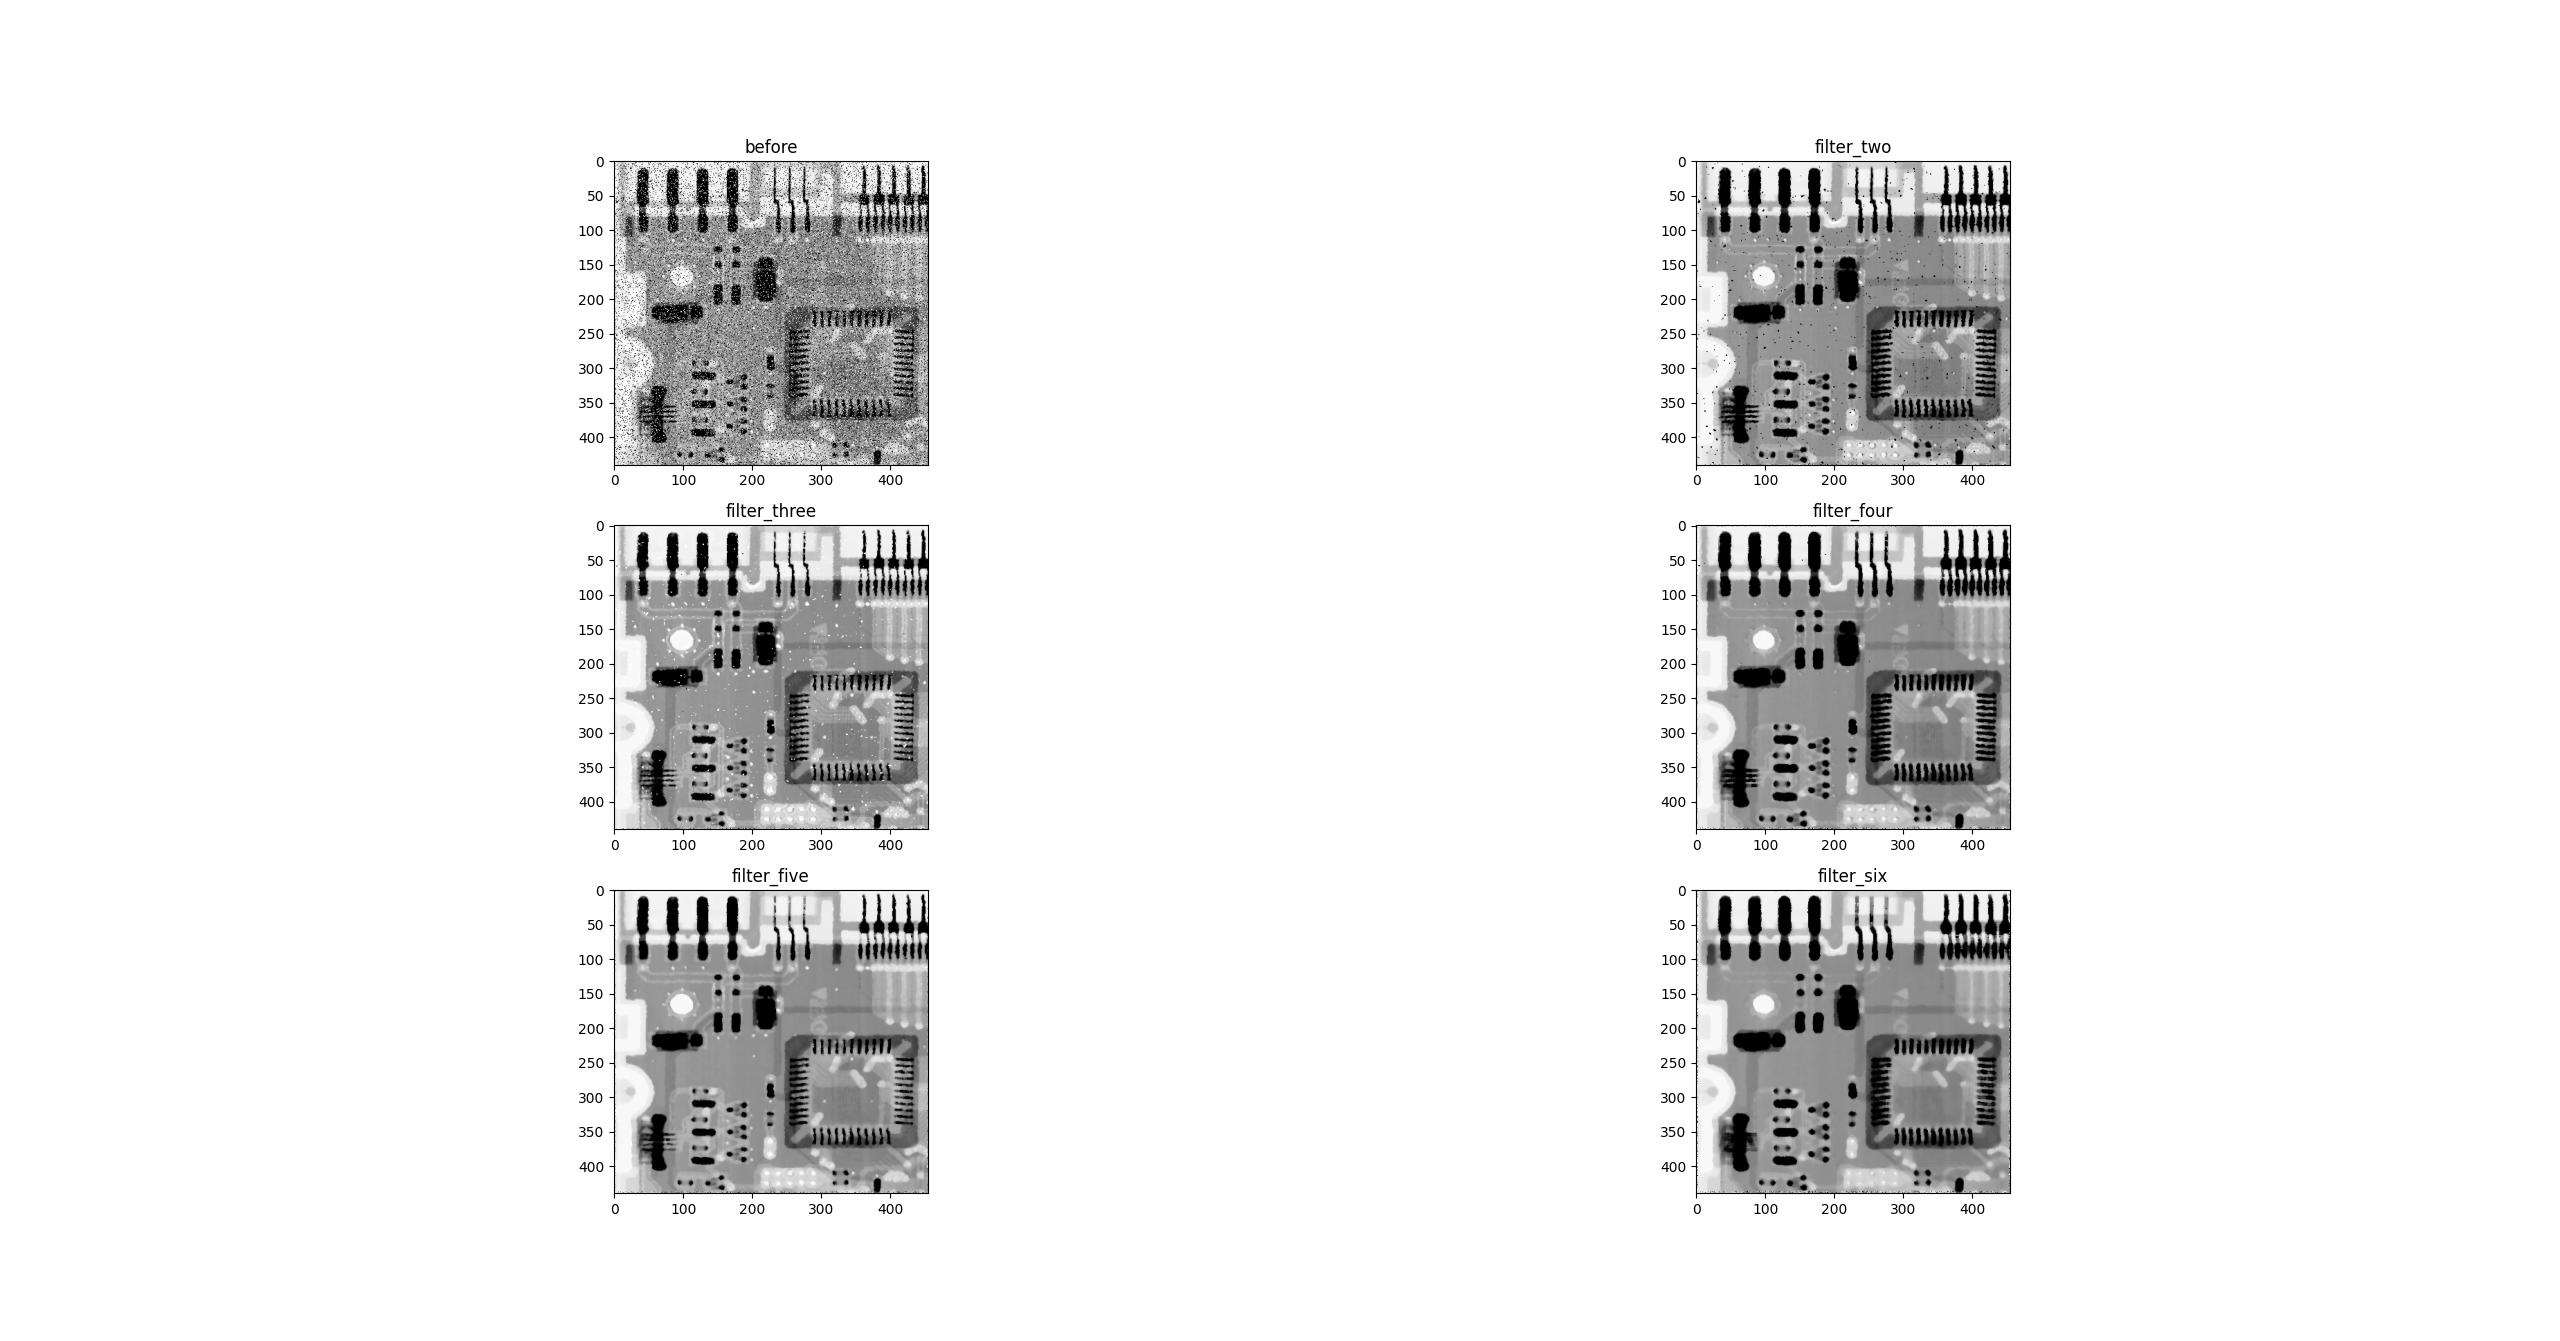
\includegraphics[scale=0.2]{contrast.png}
                \caption{结果}
            \end{figure}

\end{document}
